\documentclass{beamer}
\usetheme{Madrid}
\usepackage[utf8]{inputenc}
\usepackage[T1]{fontenc}
\usepackage{graphicx}
\usepackage{lmodern}

% Pour enlever le \institute du bas de page
% Rapetisser les noms et date etc dans le footer
\setbeamertemplate{footline}
{
	\leavevmode%
	\hbox{%
	\begin{beamercolorbox}[wd=.333333\paperwidth,ht=2.25ex,dp=1ex,center]{author in head/foot}%
	\
	\end{beamercolorbox}%
	\begin{beamercolorbox}[wd=.333333\paperwidth,ht=2.25ex,dp=1ex,center]{title in head/foot}%
	\usebeamerfont{title in head/foot}\insertshorttitle
	\end{beamercolorbox}%
	\begin{beamercolorbox}[wd=.333333\paperwidth,ht=2.25ex,dp=1ex,right]{date in head/foot}%
	\usebeamerfont{date in head/foot}\insertshortdate{}\hspace*{2em}
	\insertframenumber{} / \inserttotalframenumber\hspace*{2ex} 
	\end{beamercolorbox}}%
	\vskip0pt%
}

\AtBeginSection[]
{
	\begin{frame}
		\tableofcontents[currentsection,hideallsubsections]
	\end{frame}
}

\title{Soutenance Projet TER}
\author{Baptiste Saleil, Geoffrey Mélia, Julien Pagès, Kevin Bollini}
\date{25 avril 2012}

\begin{document}
	\begin{frame}
		\titlepage
	\end{frame}

	%Plan
	\begin{frame}{Plan}
		\tableofcontents
	\end{frame}

	\section{Introduction}
		\begin{frame}{Introduction}
		\begin{center}
		\LARGE{Ter de Master 1 : Tableau virtuel interactif}
		\end{center}
		
		But du projet :
		\begin{itemize}
		\item Concevoir une application avec une interface naturelle (mouvements)
		\item Librairie de reconnaissance de mouvements
		\item Application pour exploiter cette librairie pour dessiner ou écrire
		\end{itemize}
		
		\end{frame}

		
	\section{Analyse et Conception}
	\subsection{Choix de conceptions}
		\begin{frame}{Choix de conceptions}
			
			\begin{block}{Choix principal}
				- Découper en deux parties distinctes le projet \\
				- Librairie réutilisable \\
				- Application sur une interface naturelle exploitant cette librairie \\
			\end{block}
			
		\end{frame}
		
	\subsection{Gestion de projet}
		\begin{frame}{Gestion de projet}
		Organisation :
			\begin{itemize}
				\item{Réunions}
				\item{Deux sous-groupes}
				\item{Partage des tâches au sein des groupes}
				\item{Choix groupés (à quatre)}
			\end{itemize}
		
		Collaboration :
			\begin{itemize}
				\item{Gestionnaire de version (Subversion)}
				\item{Partage de documents (Mail et Subversion)}
				\item{Discussions (Mails / Instantanée)}
				\item{Édition collaborative pour le travail à distance (Gobby)}
			\end{itemize}
		\end{frame}
		
		\begin{frame}{Gestion de projet}
			Objectif :
			\begin{itemize}
			\item Se renseigner, faire une bonne architecture
			\item Développer rapidement un prototype
			\item Développement incrémental en ajoutant des fonctionnalités
			\end{itemize} 
		\end{frame}
		
		\begin{frame}{Rétroplanning}	
			Rétroplanning (Diagramme de gantt) :
			\begin{center}
			% TODO : mettre à jour le rétroplanning
			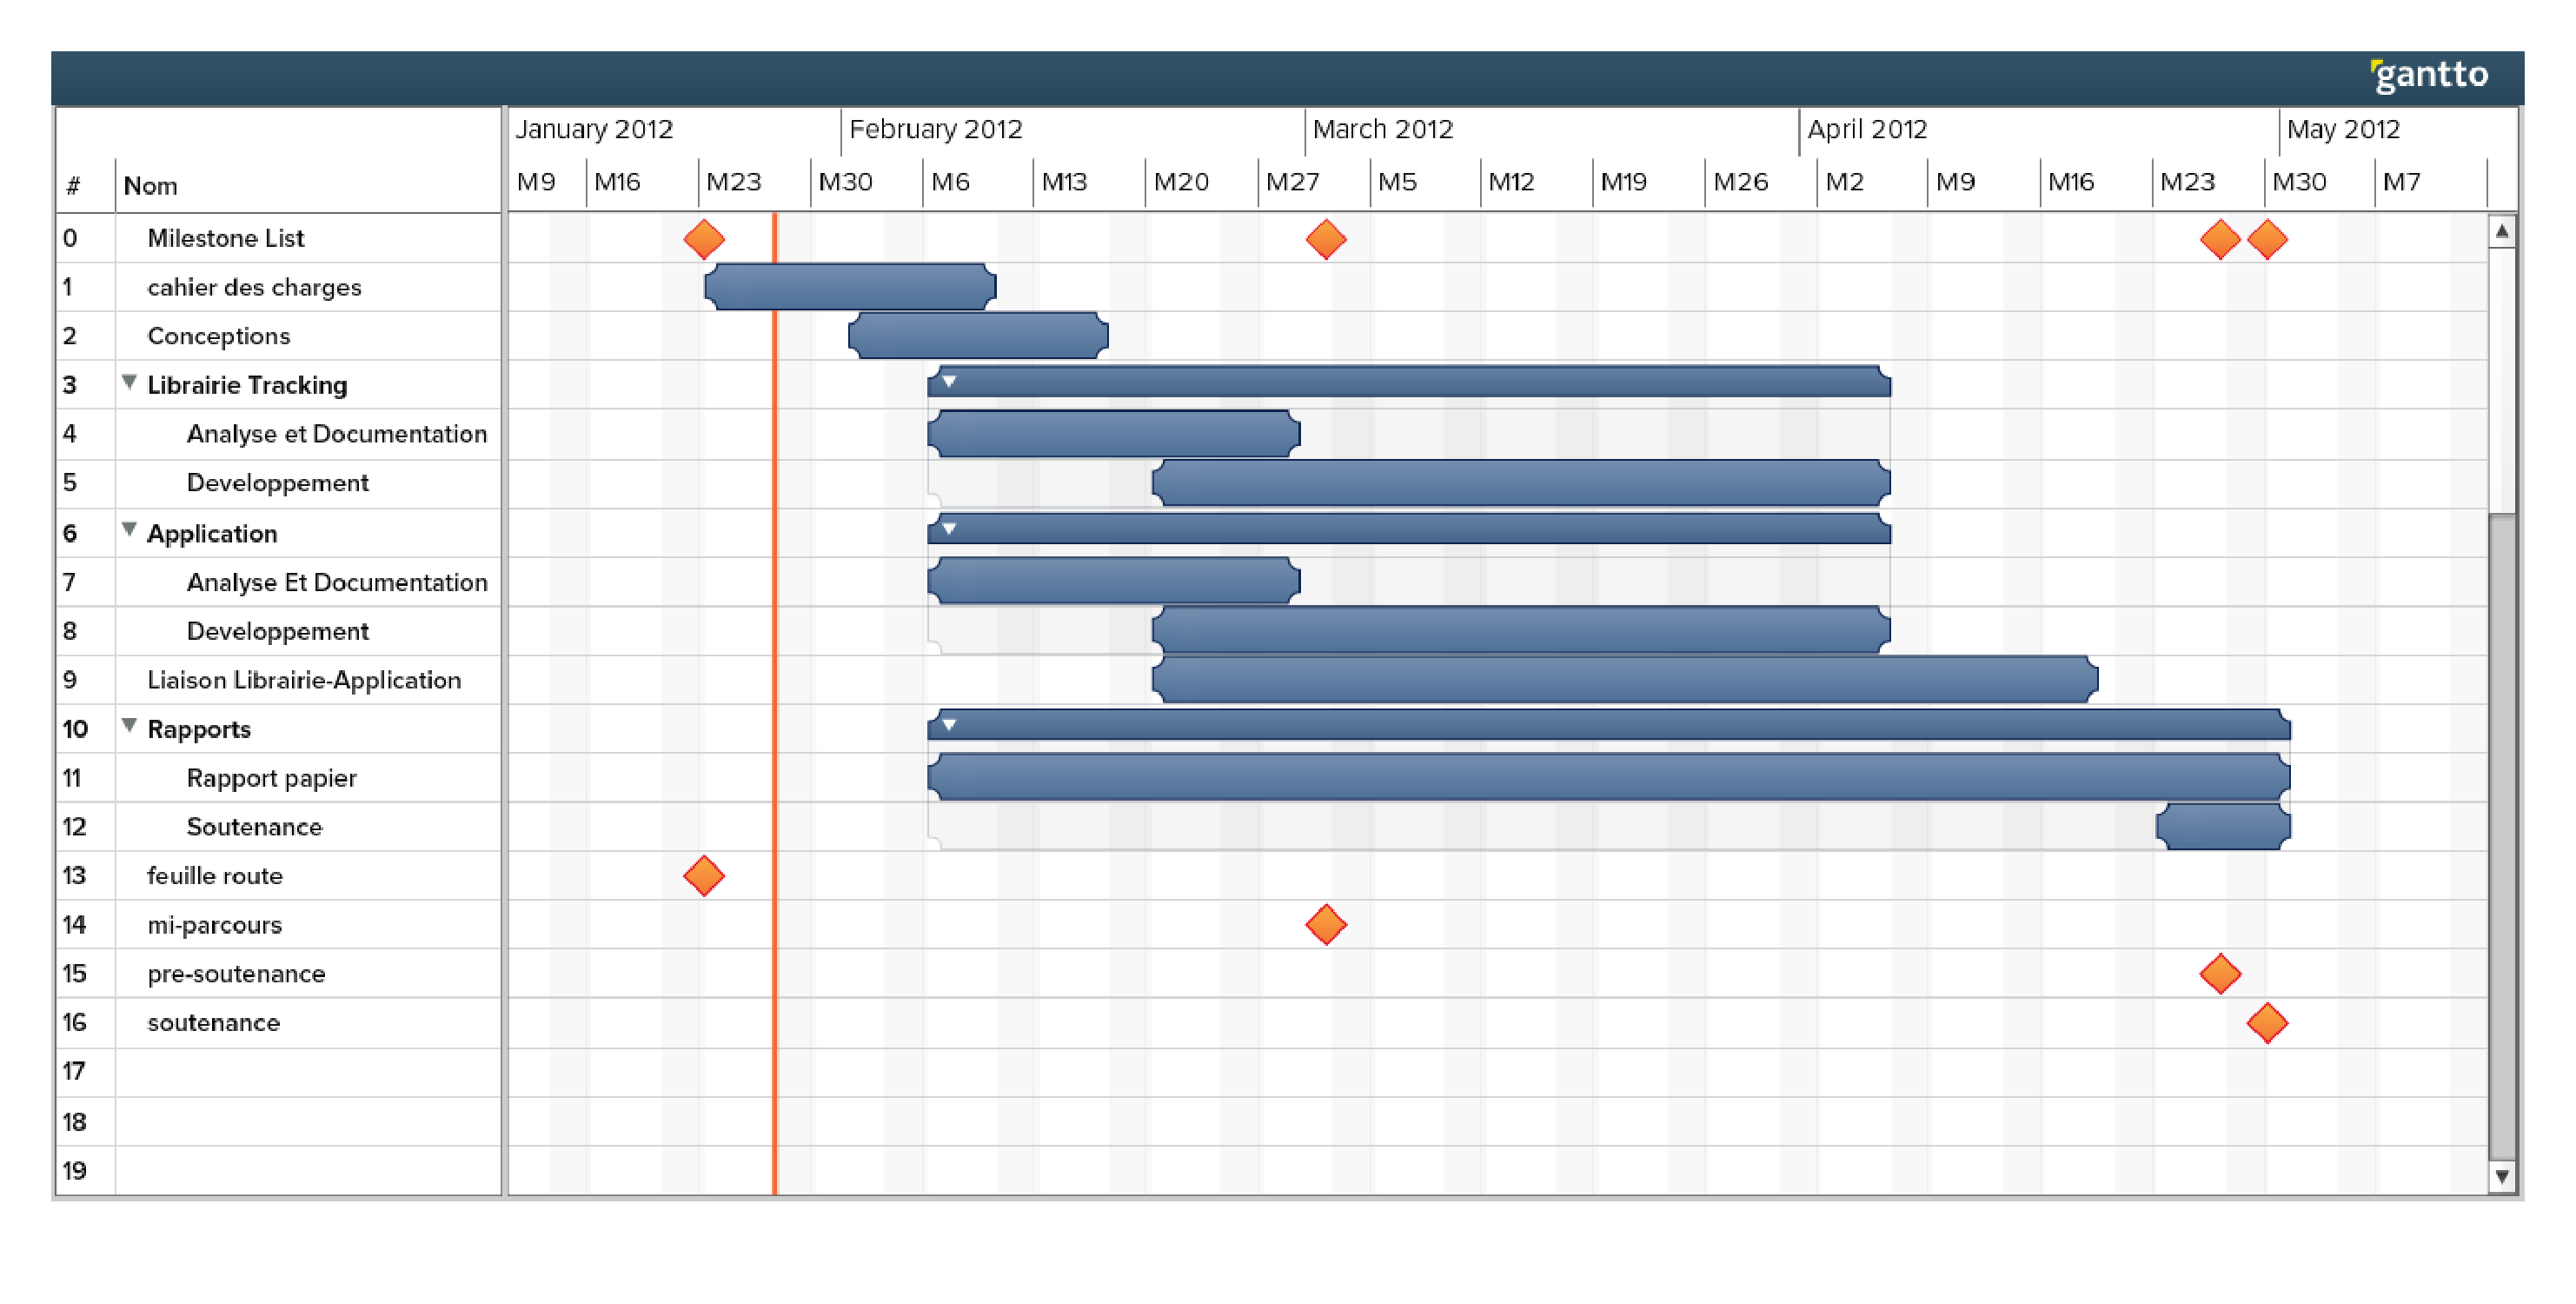
\includegraphics[scale=0.25]{../feuille-route/retroplanning.pdf}
			\end{center}
		\end{frame}
	
	\subsection{Analyse}
		\begin{frame}{Analyse}
				\begin{exampleblock}{Objectifs}
				\begin{itemize}
					\item{Identifier les besoins et envies potentielles des utilisateurs}
					\item{Distinguer et classer les fonctionnalités de l'application}
					\item{Etablir un schéma de conception dans le temps}
					\item{Faciliter le développement, permets d'avoir des buts concrets}
				\end{itemize}
				\end{exampleblock}
		\end{frame}
	
	\section{Librairie}
		
		\begin{frame}{Librairie}
		Deux types de suivis ont été développés : \\
				\begin{itemize}
					\item{Traçage par couleur}
					\item{Traçage par forme}
				\end{itemize}
		\end{frame}

		\subsection{Traçage par Couleur}
		\begin{frame}{Étalonnage}
				\begin{itemize}
					\item{Sélection de l'objet}
					\item{Détection de couleur}
				\end{itemize}
		\end{frame}

		\begin{frame}{Traçage}
				\begin{itemize}
					\item{Centre de gravité de l'image binaire}
					\item{Librairie CVBlob}
				\end{itemize}
		\end{frame}

		\subsection{Traçage par Forme}
		\begin{frame}{Etalonnage}
				\begin{itemize}
					\item{Sélection de l'objet}
					\item{Sous-image Template}
				\end{itemize}
		\end{frame}

		\begin{frame}{Traçage}
				\begin{itemize}
					\item{Recherche du Template}
				\end{itemize}
		\end{frame}
	
	
	\section{Application}
		\begin{frame}{Architecture}
			\begin{block}{Objectifs de l'architecture conçue}
				\begin{itemize}
				\item{Avoir une application modulable et facilement extensible}
				\item{Fonctionnement identique pour les classes principales en réseau ou en local}
				\item{Pouvoir rajouter facilement des outils}
				\item{Séparer le traitement du rendu}
				\end{itemize}
			\end{block}
		\end{frame}
		
		\begin{frame}{Diagramme de classes}
			\begin{center}		
			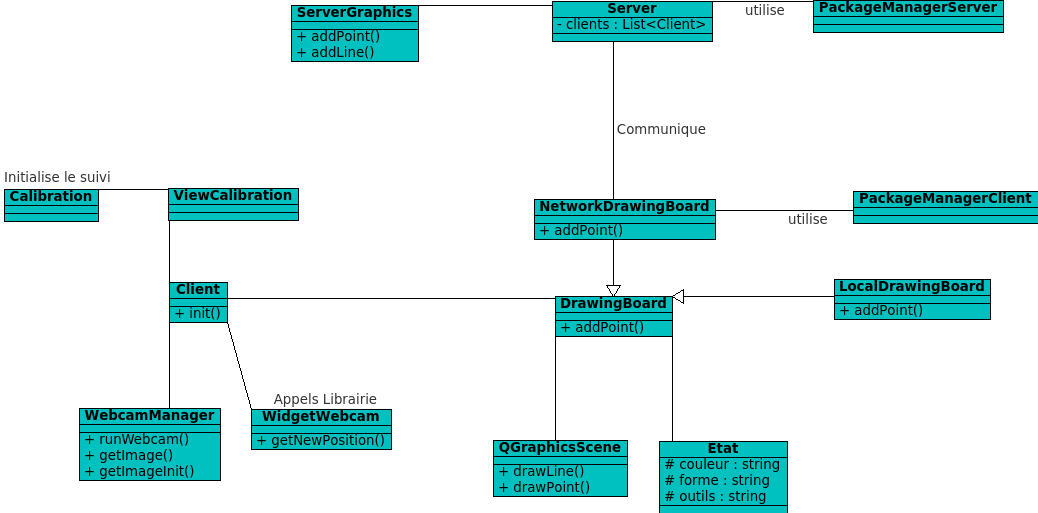
\includegraphics[scale=0.45]{../uml/classes.png}
			\end{center}
		\end{frame}
		
		\begin{frame}{Application}
			
			L'application est utilisable en local et en réseau, avec un fonctionnement identique.
			
			% TODO : écrire les fonctionnalités voulues
		\end{frame}
		
	\subsection{Module Local}
		\begin{frame}{Aperçu}
			\begin{block}{Fonctionnement en local}
				\begin{itemize}
				\item Étalonnage selon la méthode voulue, choix du mode local
				\item Détection d'un mouvement, dessin directement sur le tableau en respectant les options
				\end{itemize}
			\end{block}
		\end{frame}
		
		\begin{frame}{Étalonnage}
		\end{frame}
		\begin{frame}{Dessin}
		\end{frame}

	\subsection{Module Reseau}
		\begin{frame}{Aperçu}
		\begin{block}{Fonctionnement en réseau}
			\begin{itemize}
			\item Étalonnage selon la méthode voulue, choix du mode réseau
			\item Récupération du dessin actuel par le client
			\item Détection d'un mouvement
			\item Envoi au serveur de ce mouvement (et des options) en respectant le protocole
			\item Réception du paquet côté serveur, dessin du serveur
			\item Envoi aux clients de ce point déssiné avec les options
			\item Réception côté client, et dessin en local
			\end{itemize}
		\end{block}
		\end{frame}
		
		\begin{frame}{Client}
		\end{frame}
		\begin{frame}{Serveur}
		\end{frame}

	\section{Conclusion}
		\begin{frame}{Conclusion}
			\begin{alertblock}{Difficultés}
				- Collaboration \\
				- Formation \\
				- Technique 
			\end{alertblock}
			\pause
			\begin{exampleblock}{Objectifs atteints}
				- Solution fonctionnelle \\
				- Respect du cahier des charges \\
				- Découverte (Objet, Technologies,...) 
			\end{exampleblock}
			\pause
			\begin{block}{Ouverture}
				- Diversifier les methodes de tracking\\
				- Optimiser les IHM \\
			\end{block}
		\end{frame}
	
	\begin{frame}
		\begin{center}
			\huge{Merci pour votre attention.} \\
		\end{center}
	\end{frame}

\end{document}
